\documentclass[t,compress,aspectratio=169]{beamer}
\include{preamble}

\title{The Art of Logging}
\subtitle{How to get helpful error reports}
\author{Andreas Cord-Landwehr}
\newcommand{\authoremail}{cordlandwehr@kde.org}

\definecolor{BreezeGray}{RGB}{77,77,77}
\definecolor{BreezeBlack}{RGB}{0,0,0}

\definecolor{KDEdarkblue}{RGB}{0,58,128}
\definecolor{KDElightblue}{RGB}{144,196,231}
\definecolor{KDElightgray}{RGB}{208,209,211}

\definecolor{KDEgray1}{RGB}{105,106,107}
\definecolor{KDEgray2}{RGB}{159,160,162}
\definecolor{KDEgray3}{RGB}{208,209,211}
\definecolor{KDEgray4}{RGB}{237,237,238}

\definecolor{KDEred}{RGB}{237,21,21}
\definecolor{KDEorange}{RGB}{246,116,0}
\definecolor{KDEblue}{RGB}{61,174,233}
\definecolor{KDEturquois}{RGB}{28,220,154}
\definecolor{KDEgreen}{RGB}{17,209,22}

\lstset{ %
  language=C++,
%   backgroundcolor=\color{KDEgray4},
%   basicstyle=\footnotesize\ttfamily,
%   breakatwhitespace=false,
%   breaklines=true,
%   captionpos=b,
%   commentstyle=\color{KDEgreen},
%   escapeinside={\%*}{*)},
%   extendedchars=true,
%   frame=single,
   keywordstyle=\color{KDEblue},
%   language=Prolog,
%   numbers=left,
%   numbersep=5pt,
%   numberstyle=\tiny\color{lightgray},
%   rulecolor=\color{lightgray},
%   showspaces=false,
%   showstringspaces=false,
%   showtabs=false,
%   stepnumber=1,
   stringstyle=\color{KDEorange},
%   tabsize=2,
%   title=\lstname,
  morekeywords={QCOMPARE, QVERIFY, QFINDTESTDATA, QFETCH, Q_EXPECT_FAIL, QTEST_MAIN},
%   deletekeywords={time}
}

\begin{document}

\usebackgroundtemplate{\includegraphics[height=\paperheight]{1920x1080-akademy}}
\begin{withoutheadline}
\begin{frame}
\titlepage
\end{frame}
\end{withoutheadline}
\usebackgroundtemplate{
\includegraphics[height=\paperheight]{1920x1080-noakademy}}

%==============================================================================

\section{Part 1: Introduction}

\begin{frame}
    {About me}

    \begin{itemize}
        \item I am Andreas (nick: CoLa) and I am with KDE for about a decade
        \item In my day job, I am working on software for big agriculture vehicles
    \end{itemize}
    \bigskip
    \pause

    \textbf{My Motivation for this Talk}
    \begin{itemize}
        \item Getting a bug report without proper logs is frustrating, especially when you cannot reproduce it
        \item I get annoyed when I start an application and see tons of non useful (for me in a user perspective) log messages
        \item Time is valuable and you should not waste it by spending too much time on reading logs to analyze a problem
        \item \dots and I think that doing logging correctly is easy :D
    \end{itemize}
\end{frame}

\begin{frame}
    {Developer Logs}

    Log messages are text lines that are printed by the a program when something ``meaningful'' happens
    \medskip

    \textbf{Examples:}
    \begin{itemize}
        \item something happened that should not happen
        \item output the helps to follow program logic and where a developer can analyze if steps fit to his thinking
        \item tracking of user interactions in order to make an error analysis possible
        \item tracing points (mostly out of scope here)
    \end{itemize}
    \medskip

    Usually, logs are printed to stdout -- at the end of the talk I will show alternatives
\end{frame}

\begin{frame}
    {Log Message Severity Levels}

    \begin{description}
        \item[Fatal] Something so critical happened that you only print a log message and then die.
        \item<2->[Critical] Something bad happened and an operation could not be performed; possibly with data loss.
        \item<3->[Warning] Something unexpected/unwanted happened but the program can resume and handle this situation.
        \item<4->[Info] A low frequent change in the programs business state done by user or by data.
        \item<5->[Debug] Messages that print information for ``interesting'' program locations and help you to see what happened.
        \item<6->[Trace] High frequent debug messages that can be activated to deeply analyse specific operations.
    \end{description}
\end{frame}

\section{Part 2: The Qt Logging Framework in KDE}

\begin{frame}[fragile]
    {QDebug}
    {Stream-API (there is also printf API, but I will only use stream API in the following)}

    \begin{columns}

    \column[T]{.50\textwidth}
    \begin{minipage}{.95\linewidth}
    \begin{lstlisting}
    #include <QDebug>
    qDebug() << "welcome!";
    // welcome!
    qWarning() << QDate::currentDate();
    // QDate("2021-06-20")
    qCritical() << QRect(1, 2, 3, 4);
    // QRect(1,2 3x4)
    int year = 2021;
    qDebug() << "Akademy" << year;
    // Akademy 2021
    qDebug().nospace().noquote()
        << "Akademy" << year;
    // Akademy2021
    qDebug() << Qt::hex
        << Qt::uppercasedigits << year;
    // 7E5
    \end{lstlisting}
    \end{minipage}

    \column[T]{.50\textwidth}
    \begin{itemize}
        \item log severity: \texttt{qDebug}, \texttt{qWarning}, \texttt{qInfo}, \texttt{qCritical}, \texttt{qFatal}
        \item<2-> support for \textbf{many} Qt data types with pretty printing
        \item<3-> you can also register your own debug printers for your data type
        \item<4-> simple output assembly
        \item<5-> \texttt{QDebugStateSaver} for resetting stream format state
        \item<6->[$\rightarrow{}$] \url{https://doc.qt.io/qt-5/qdebug.html}
    \end{itemize}
    \end{columns}
\end{frame}

%TODO shall QML debug be also in scope?

\begin{frame}[fragile]
    {Categorized Logs}
    {The better way}

    Group log messages by hierarchical categories:
    \begin{center}
        \texttt{category.subcategory.subsubcategory.[\dots]}
    \end{center}

    Log outputs can be enabled/disabled at runtime by category and message type.
    \medskip

    \pause
    \textbf{Define Global Logging Categories}
    \begin{verbatim}
Q_DECLARE_LOGGING_CATEGORY(name) // declare it in header

// define category and make it usable with string identifier
Q_LOGGING_CATEGORY(name, string)
// optional msgType sets enabled minimal severity
Q_LOGGING_CATEGORY(name, string, msgType)
    \end{verbatim}
\end{frame}

\begin{frame}[fragile]
    {Categorized Logs}
    {Example}

    \texttt{loggingcategories.h}
    \begin{minipage}{.95\linewidth}
    \begin{lstlisting}
    #pragma once
    #include <QLoggingCategory>
    Q_DECLARE_LOGGING_CATEGORY(mycoolcategory);
    \end{lstlisting}
    \end{minipage}
    \medskip

    \texttt{loggingcategories.cpp}
    \begin{minipage}{.95\linewidth}
    \begin{lstlisting}
    #include "loggingcategories.h"
    Q_LOGGING_CATEGORY(mycoolcategory, "myapp.foo", QtWarningMsg);
    \end{lstlisting}
    \end{minipage}
    \medskip

    Just using it:
    \begin{minipage}{.95\linewidth}
    \begin{lstlisting}
    #include "loggingcategories.h"
    qCDebug(mycoolcategory) << "log message in category myapp.foo";
    \end{lstlisting}
    \end{minipage}
\end{frame}

\begin{frame}[fragile]
    {Log Filtering}

    Assume we have an app \texttt{myapp} with logging categories:

    \begin{enumerate}
        \item \texttt{<QLibraryInfo::DataPath>/qtlogging.ini}, \texttt{[Rules]} section
        \item \texttt{.config/QtProject/qtlogging.ini}, \texttt{[Rules]} section
        \item \texttt{setFilterRules(const QString \&rules)}
        \item \texttt{[Rules]} section of file set in \texttt{QT\_LOGGING\_CONF}
        \item \texttt{QT\_LOGGING\_RULES} environment variable
    \end{enumerate}
    \bigskip

    Output filtering with \texttt{QT\_LOGGING\_RULES} variable:

    \begin{minipage}{.95\linewidth}
    \begin{lstlisting}
QT_LOGGING_RULES=*=true ./myapp # we see everything
QT_LOGGING_RULES=myapp.lib=true,myapp.backend=false ./myapp # only lib, no backend
    \end{lstlisting}
    \end{minipage}
\end{frame}

\begin{frame}[fragile]
    {Logging Rules Format}

    \begin{columns}
    \column[T]{.50\textwidth}
    \texttt{category[.type] = true|false}
    \medskip

    \begin{minipage}{.95\linewidth}
    \begin{lstlisting}
    *=true
    kate.*=false
    kwrite.debug=true
    *.critical=true
    *.strangethings.*=true
    \end{lstlisting}
    \end{minipage}

    \column[T]{.50\textwidth}
    \textbf{Rule Formats}\\
    \begin{itemize}
        \item type can be any of: debug, info, warning, critical
        \item $*$ wildcard only allowed as first and/or last character
        \item rules evaluated from first to last
    \end{itemize}
    \end{columns}
\end{frame}


\begin{frame}
    {User Friendly Log Filtering}

    \vspace{-0.2em}
    Use \texttt{kdebugsettings} to edit \texttt{.config/QtProject/qtlogging.ini}:

    \begin{center}
    \noindent\includegraphics[width=0.4\textwidth]{kdebugsettings.png}
    \end{center}

    \textbf{Note:} To allow configuration, you have to install the logging category names though! (\texttt{/usr/share/qlogging-categories5/})
\end{frame}

\begin{frame}[fragile]
    {Using Extra-CMake-Modules}

    \url{api.kde.org/ecm/module/ECMQtDeclareLoggingCategory.html}

    \begin{minipage}{.95\linewidth}
    \begin{lstlisting}
ecm_qt_declare_logging_category( MYPROJECT_SRCS
    HEADER "myproject_debug.h"
    IDENTIFIER "MYPROJECT_DEBUG"
    CATEGORY_NAME "myproject"
    OLD_CATEGORY_NAMES "myprojectlog"
    DESCRIPTION "My project"
    EXPORT MyProject
)
ecm_qt_export_logging_category( IDENTIFIER "MYPROJECT_SUBMODULE_DEBUG"
    CATEGORY_NAME "myproject.submodule"
    DESCRIPTION "My project - submodule"
    EXPORT MyProject
)
ecm_qt_install_logging_categories( EXPORT MyProject
    FILE myproject.categories
    DESTINATION "${KDE_INSTALL_LOGGINGCATEGORIESDIR}"
)
    \end{lstlisting}
    \end{minipage}
\end{frame}

\section{Part 3: Log Sinks}

\begin{frame}
    {Logging Sinks}
    {Perspective = we look at a full system with many apps}

    \textbf{Question:} How to store logs and serialize async log outputs?
    \begin{columns}
    \column[T]{.50\textwidth}
    \begin{itemize}
        \item Qt supports several log backend integrations apart from stdout
        \item backend selected at Qt configure time (eg. Fedora enables journald)
        \item when enabled, such log databases can be super helpful
        \item \dots unless there are too many logs
    \end{itemize}

    \column[T]{.50\textwidth}
    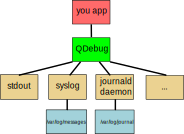
\includegraphics[width=.9\textwidth]{logsinks}
    \end{columns}
    \medskip

    \textbf{Note:} Per default journald forwards system session logs to syslog
\end{frame}


\begin{frame}
    {journald}
    {I like it}

    \begin{itemize}
        \item Internal log rotation and file consistency checks
        \item Pretty robost database files with internal index handling for fast usage
        \item Awesome CLI tool: \texttt{journalctl}:
            \begin{enumerate}
                \item \texttt{journalctl -b 1} : only last boot's logs
                \item \texttt{journalctl -u sddm} : only log of \texttt{sddm} systemd service
                \item \texttt{journalctl -u sddm -p 1..4} only \texttt{sddm} output up to warning
                \item \dots and much more
            \end{enumerate}
    \end{itemize}
    \medskip

    \pause
    \textbf{Remarks for Integration}
    \begin{itemize}
        \item for Qt only one backend must be configured at once (default = none)
        \item when backend is configured, you do not see console output unless: \texttt{QT\_FORCE\_STDERR\_LOGGING=1}
        \item systemd services (thanks @Plasma team!) are nicely integrated
    \end{itemize}

\end{frame}

\begin{frame}
    {journald with colors and filters}
    {Suggestion for nicer integration}

    \url{https://invent.kde.org/libraries/kjournald}
    \begin{itemize}
        \item goal: QAbstractItemModel abstraction of journald's C-API
        \item allows trivial integration into applications: I am looking for a nice use case in KDE :)
        \item ships a reference implementation for a QtQuick based journald browser
            \begin{enumerate}
                \item filter by boots, systemd services and severity
                \item rainbow colors for services
            \end{enumerate}
        \item my main use case right now: offline analysis of journald databases from embedded devices $\rightarrow$ could this be helpful for Plasma mobile, too?
    \end{itemize}
\end{frame}

\begin{frame}
    {kjournald-browser}
    \centering
    \vspace{-2.5em}
    \includegraphics[width=.8\textwidth]{kjournaldbrowser}
\end{frame}

\section{The End}
\begin{frame}{Key Messages}
    \begin{block}{Please take this home}
        \begin{itemize}
            \item Only use categorized logging
            \item Add all meaningful log messages you want
            \item Disable verbose logs per default (set level to eg. Warning or Info)
            \item For bug reports you can tell users to enable more logs
            \item Start \texttt{journalctl} or kjournald-browser and look at your own system
        \end{itemize}
    \end{block}
    \bigskip

    \textbf{Skipped due to time:} you can format your output messages as you like\\
    $\rightarrow$ \url{https://doc.qt.io/qt-5/debug.html}
\end{frame}


\begin{frame}
    \frametitle{The End}
    \vspace{0.3cm}
    \begin{block}{}
        \centering\begin{Huge}Question Time\end{Huge}
    \end{block}
    \vspace{1.1cm}
    \begin{tiny}
        \begin{block}{Contact}
            \begin{description}
%                 \item[Project Name] \url{http://your.url/}\\ \url{http://another.url/}\\ irc: \#channelname on freenode
                \item[Contact] mail: \url{cordlandwehr@kde.org} \\irc: CoLa
            \end{description}
        \end{block}
    \end{tiny}
\end{frame}

\end{document}
